\section{Résultats expérimentaux}

Les fonctions dont nous nous sommes servi pour tester le programme se trouvent
dans le fichier \texttt{test.c}. Nous avons effectué nos tests sur des entiers
générés par la fonction \texttt{rand\_N}. Ces entiers sont de la forme $N = pq$
avec $p$ et $q$ des premiers aléatoires et de taille semblable. 

\subsection{Choix de la taille de la base de factorisation}

Nous avons cherché à déterminer expérimentalement, selon la taille de l'entier
$N$ à factoriser, une bonne taille pour la base de factorisation lorsque la \textit{large
prime variation} et la \textit{early abort strategy} sont utilisées. Pour une
taille d'entier fixée, nous avons inscrit dans un fichier le temps que met le
programme pour plusieurs tailles de bases de factorisation.
Nous donnons ci-dessous des tailles appropriées (il ne s'agit que d'un
ordre de grandeur, la taille optimale varie d'un entier à l'autre). Ce sont
elles qui sont renvoyées par la fonction \texttt{choose\_s\_fb}.

\begin{center}
    \begin{tabular}{ |l |l | }
        \hline
         nombre de bits de $N$ & taille de la base de factorisation \\ \hline
         70                    & 40                                 \\ \hline
         80                    & 90                                 \\ \hline
         90                    & 120                                \\ \hline 
         100                   & 170                                \\ \hline 
         110                   & 260                                \\ \hline 
         120                   & 280                                \\ \hline 
         130                   & 370                                \\ \hline 
         140                   & 450                                \\ \hline 
    \end{tabular}
\end{center}

\subsection{Factorisation de $F_7$}

Notre programme permet de factoriser $F_7 = 2^{128} + 1$. La fonction 
\texttt{fact\_F7} prend en entrée des booléens indiquant si la
\textit{large\_prime variation (lp)} et la \textit{early abort strategy (eas)}
doivent être utilisées et lance cette factorisation. Avec le paramètre \texttt{k}
retourné par la fonction \texttt{choose\_k} - soit $k=38$ - et les paramètres 
\texttt{eas\_cut} et \texttt{eas\_coeff} valant respectivement $50$ et $1000000$,
nous obtenons les résultats suivants :  

\begin{center}
     \begin{tabular}{| l | l| l | l | l |}
     \hline
     variantes                    & \texttt{s\_fb} & \texttt{nb\_AQp} & \texttt{last\_n} & temps de calcul  \\ \hline
     \textit{lp} et \textit{eas}  &     370        &  385             &    1338269       &   30 s           \\ \hline
     \textit{lp}                  &     370        &  385             &    1013314       &   100 s          \\ \hline
     \textit{eas}                 &     950        &  965             &    1864721       &   61 s           \\ \hline
     sans variante                &     950        &  965             &    1205664       &   317 s          \\ \hline
    \end{tabular}
\end{center}

\hspace*{1.6 cm} \footnotesize{\texttt{last\_n} est l'indice de la dernière paire $(A,Q)$
calculée.}

\subsection{Temps de calcul (avec les deux variantes) }

Ce graphique représente le temps moyen mis par le programme (sur une cinquantaine de tests)
en fonction du nombre de bits de l'entier que l'on souhaite factoriser. La
\textit{large prime variation} et la \textit{early abort strategy} ont été 
utilisées et les paramètres ont été choisis par les fonctions 
\texttt{choose\_s\_fb} et \texttt{choose\_k}.\\

\begin{figure}[h]
\begin{center}
%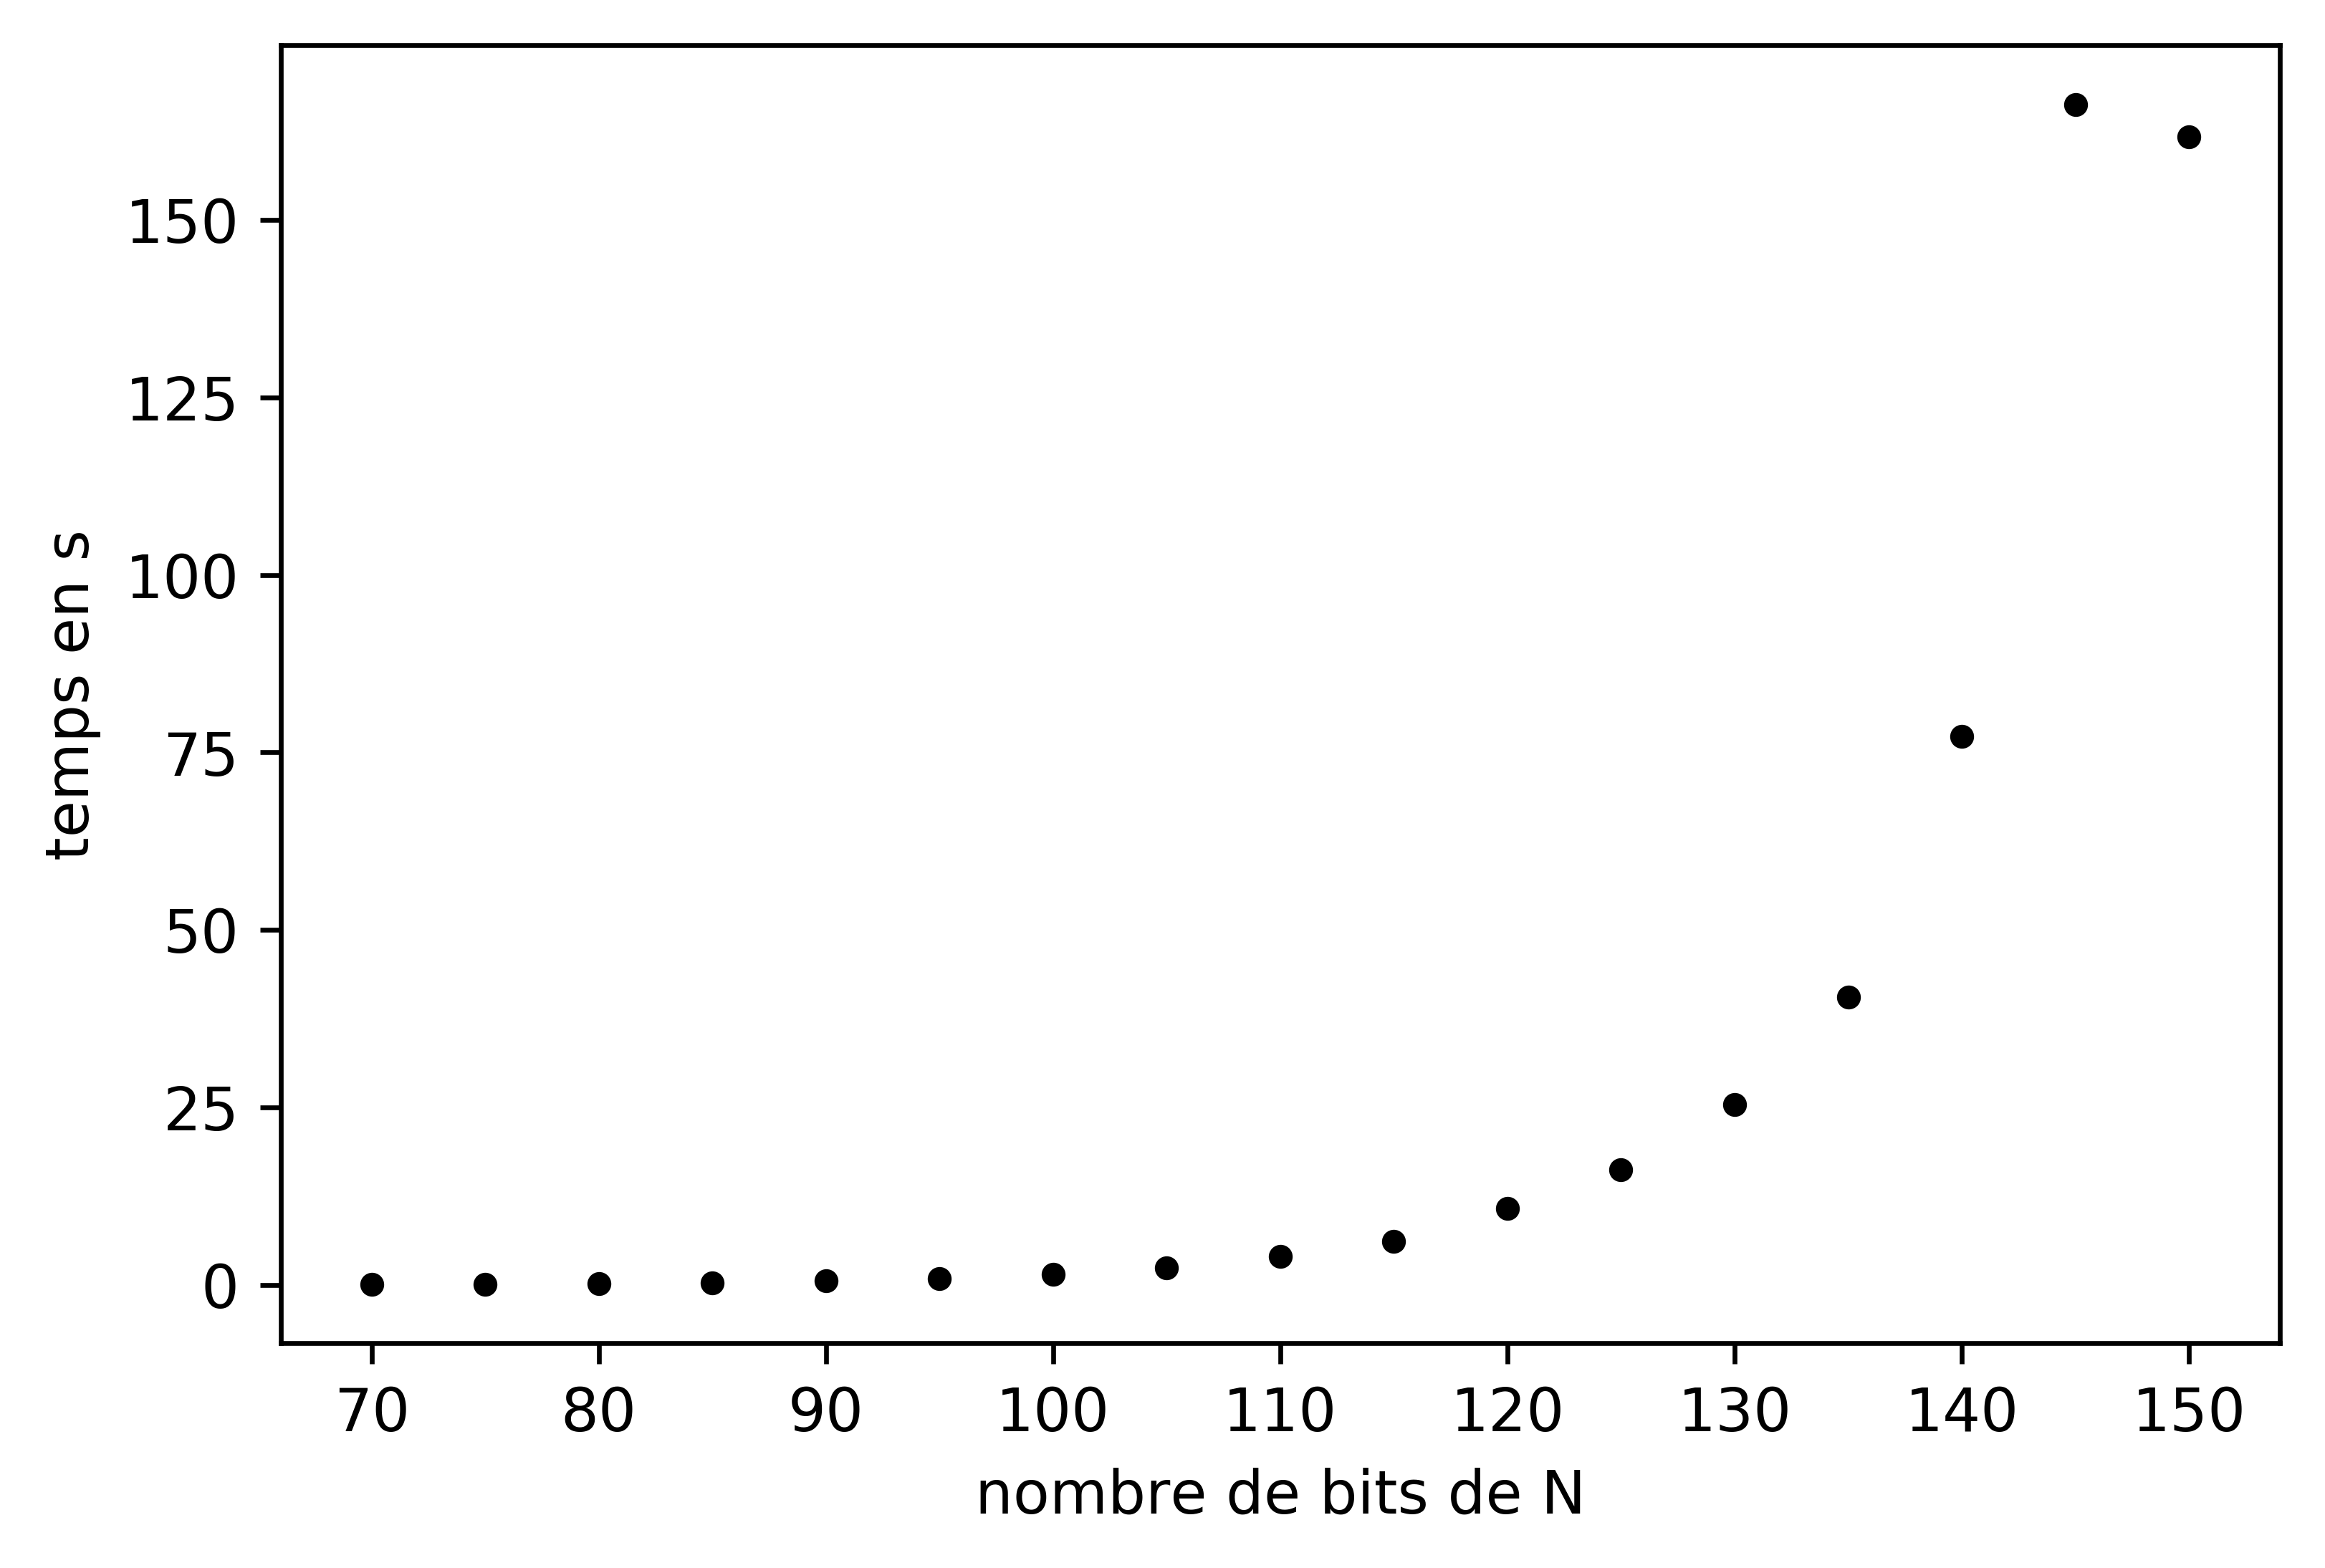
\includegraphics[width = 7 cm ]{graphique.png}
\end{center}
\end{figure}

Concernant le choix du paramètre $k$, utiliser la valeur choisie par la fonction 
\texttt{choose\_k} plutôt que $k=1$ n'améliore pas en moyenne les performances du 
programme. 
